% The recommended pipeline (solid: the evaluated configuration) and the extensions measured separately (dashed).
% Build: tectonic recommended_pipeline.tex, then render the PDF to recommended_pipeline.png (e.g. PyMuPDF, 220 dpi).
\documentclass[border=8pt]{standalone}
\usepackage[T1]{fontenc}
\usepackage{lmodern}
\usepackage{tikz}
\usetikzlibrary{positioning,arrows.meta,fit,backgrounds,calc}
\begin{document}
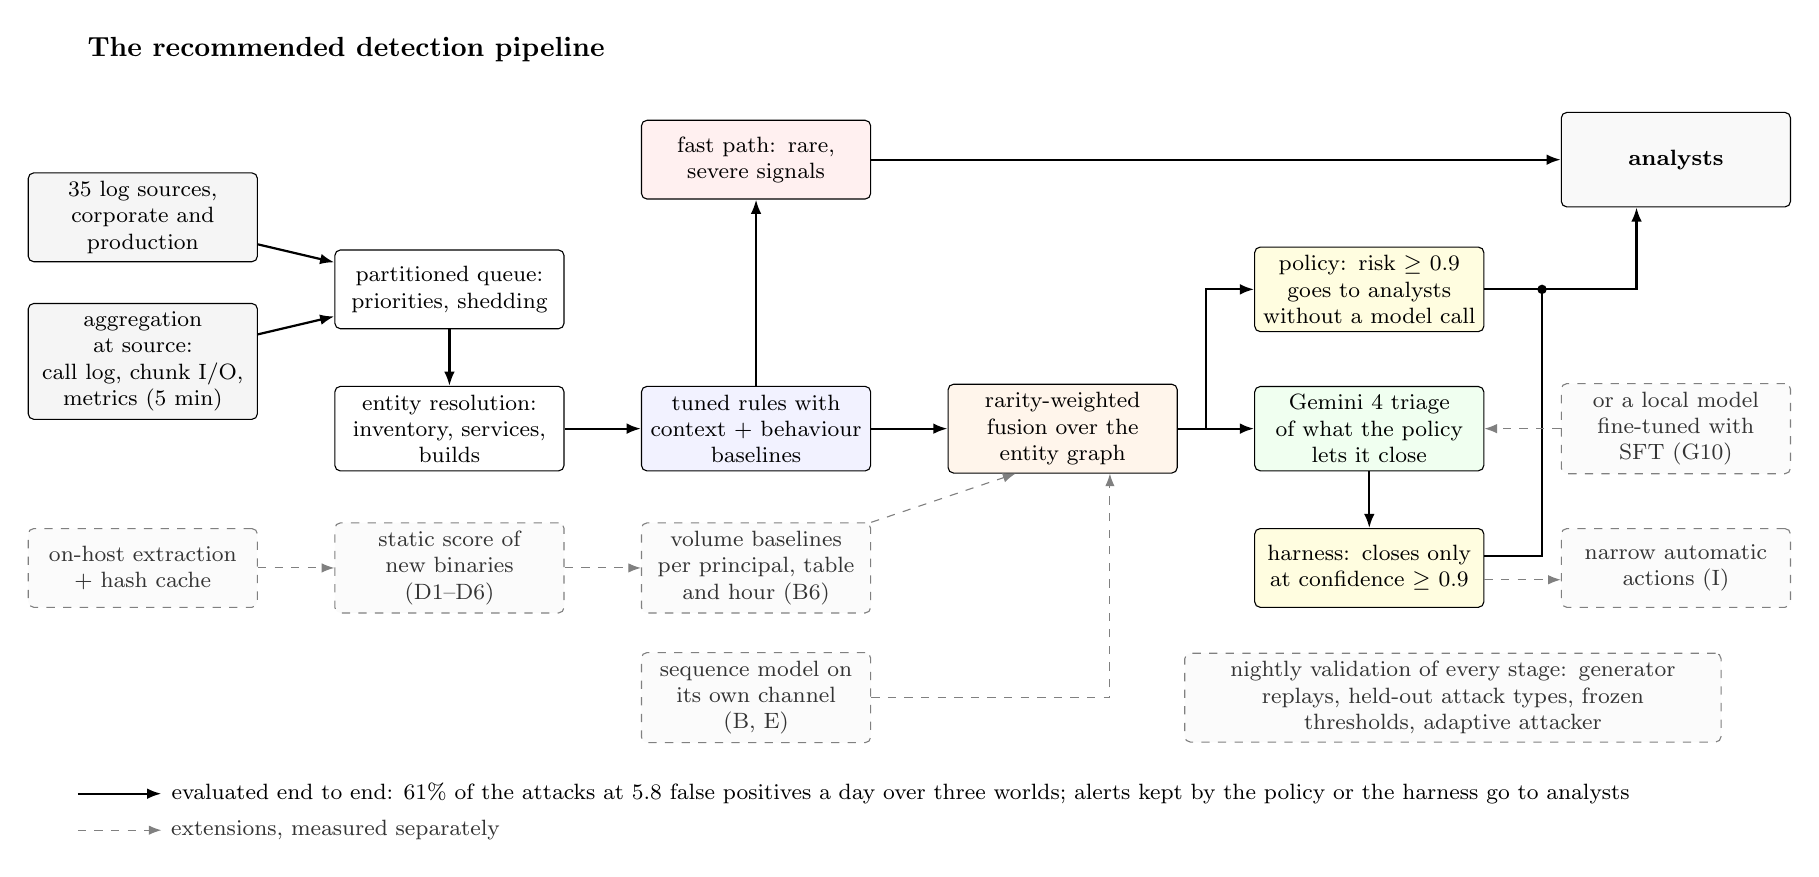
\begin{tikzpicture}[font=\footnotesize, x=1.18cm, y=1.22cm,
  box/.style={draw, rounded corners=2pt, align=center, minimum height=10mm, inner sep=3pt, fill=white, text width=27mm,
              execute at begin node={\hyphenpenalty=10000}},
  ext/.style={box, dashed, draw=gray, text=gray!40!black, fill=gray!3},
  arr/.style={-{Latex[length=1.8mm]}, thick}, darr/.style={-{Latex[length=1.6mm]}, dashed, gray}]
% evaluated pipeline
\node[box, fill=gray!8] (src) at (0,0) {35 log sources,\\corporate and\\production};
\node[box, fill=gray!8] (aggr) at (0,-1.5) {aggregation at source:\\call log, chunk I/O,\\metrics (5 min)};
\node[box] (queue) at (3.3,-0.75) {partitioned queue:\\priorities, shedding};
\node[box] (er) at (3.3,-2.2) {entity resolution:\\inventory, services,\\builds};
\node[box, fill=red!6] (fast) at (6.6,0.6) {fast path: rare,\\severe signals};
\node[box, fill=blue!5] (det) at (6.6,-2.2) {tuned rules with\\context + behaviour\\baselines};
\node[box, fill=orange!8] (fusion) at (9.9,-2.2) {rarity-weighted\\fusion over the\\entity graph};
\node[box, fill=yellow!12] (pol) at (13.2,-0.75) {policy: risk $\geq$ 0.9\\goes to analysts\\without a model call};
\node[box, fill=green!6] (llm) at (13.2,-2.2) {Gemini 4 triage\\of what the policy\\lets it close};
\node[box, fill=yellow!12] (harness) at (13.2,-3.65) {harness: closes only\\at confidence $\geq$ 0.9};
\node[box, fill=gray!5, minimum height=12mm] (analyst) at (16.5,0.6) {\textbf{analysts}};
% extensions
\node[ext] (host) at (0,-3.65) {on-host extraction\\+ hash cache};
\node[ext] (gpu) at (3.3,-3.65) {static score of\\new binaries\\(D1--D6)};
\node[ext] (vol) at (6.6,-3.65) {volume baselines\\per principal, table\\and hour (B6)};
\node[ext] (seq) at (6.6,-5.0) {sequence model on\\its own channel\\(B, E)};
\node[ext] (local) at (16.5,-2.2) {or a local model\\fine-tuned with\\SFT (G10)};
\node[ext] (act) at (16.5,-3.65) {narrow automatic\\actions (I)};
\node[ext, text width=66mm] (val) at (14.1,-5.0) {nightly validation of every stage: generator\\replays, held-out attack types, frozen\\thresholds, adaptive attacker};
% solid flow
\draw[arr] (src) -- (queue);
\draw[arr] (aggr) -- (queue);
\draw[arr] (queue) -- (er);
\draw[arr] (er) -- (det);
\draw[arr] (det) -- (fusion);
\draw[arr] (det.north) -- (fast.south);
\draw[arr] (fast) -- (analyst);
\draw[arr] (fusion.east) -- ++(0.3,0) |- (pol.west);
\draw[arr] (fusion) -- (llm);
\draw[arr] (pol.east) -| ([xshift=-5mm]analyst.south);
\draw[arr] (llm) -- (harness);
\coordinate (hj) at ($(pol.east)+(0.62,0)$);
\draw[thick] ([yshift=1.5mm]harness.east) -| (hj);
\fill (hj) circle (1.7pt);
% dashed extensions
\draw[darr] (host) -- (gpu);
\draw[darr] (gpu) -- (vol);
\draw[darr] (vol.north east) -- ([xshift=-6mm]fusion.south);
\draw[darr] (seq.east) -| ([xshift=6mm]fusion.south);
\draw[darr] (local) -- (llm);
\draw[darr] ([yshift=-1.5mm]harness.east) -- ([yshift=-1.5mm]act.west);
% title and legend
\node[anchor=west, font=\normalsize\bfseries] at (-0.7,1.75) {The recommended detection pipeline};
\coordinate (l1) at (-0.7,-6.0);
\draw[arr] (l1) -- ++(0.9,0) node[right, black] {evaluated end to end: 61\% of the attacks at 5.8 false positives a day over three
worlds; alerts kept by the policy or the harness go to analysts};
\draw[darr] ($(l1)+(0,-0.38)$) -- ++(0.9,0) node[right, gray!40!black] {extensions, measured separately};
\end{tikzpicture}
\end{document}
